\chapter{Background}

\section{Bipartite Network Projection}

Bipartite networks are a particular class of complex networks, whose nodes are divided into two sets \emph{X} and \emph{Y} and only edges between two nodes in different sets are allowed. For the convenience of directly showing the relation structure among a particular set of nodes, bipartite networks are usually compressed by one-mode projection. This means ensuring network contains nodes of only one of the two sets \emph{X} or \emph{Y}, and two \emph{X}(or alternatively \emph{Y}) nodes are connected if and only if they have at least one common neighbour \emph{Y}(or alternatively \emph{X}) node. Since bipartite networks with largely different structures can have one-mode representation, a lucid illustration of original network requires the use of some weighing method. Various weighting methods have been proposed and should be chosen with case.

In \emph{simple weighing technique} the edges are weighted directly by the number of times the common association is repeated. This method works in wide range of settings where the impact of each relation in the bipartite network has equal impact.

\begin{figure}[htb]
\centering
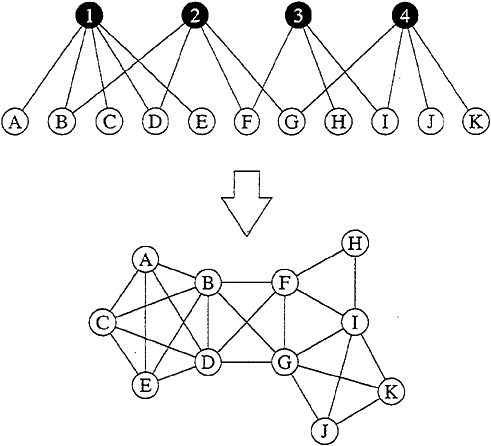
\includegraphics[scale=0.3]{bipartite} % e.g. insert ./image for image.png in the working directory, adjust scale as necessary
\caption{Bipartite network and its projection}
\label{fig:label} % insert suitable label, this is used to refer to a fig from within the text as shown above
\end{figure}

\section{Simrank}

SimRank \cite{SimRank} is an algorithm for analysing the logical graphs derived from such datasets to compare similarity scores between nodes(objects) based on \emph{structural context} in which they appear. The intuition behind this algorithm is that similar objects are related to similar objects. Consider a small directed graph as shown in the Figure \ref{fig:simrank} below. The vertices represent websites and edges represent hyperlink i.e. one website is referred by the other. The basic assumption/intuition is that two objects are similar if they are referred to by some common object. So here we can say that websites \emph{v3} and \emph{v5} are similar i.e. contain similar content because both are referred by website \emph{v2}.

\begin{figure}[htb]
\centering
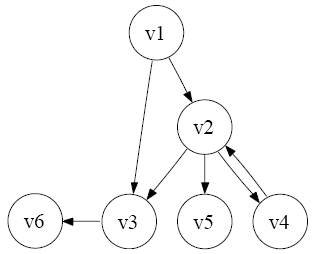
\includegraphics[scale=0.5]{simrank}
\caption{Directed graph representing websites and hyperlinks}
\label{fig:simrank}
\end{figure}

Mathematically SimRank score is defined recursively. Let us denote similarity between objects a and b by s(a, b) $\in$ [0, 1].


\begin{equation}
S(a, b) =	\left\{ \begin{array}{ll}
			1 & \mbox{if $a=b$}; \\
			\frac{C}{\left | I(a) \right | \left | I(b) \right |}\sum_{i = 0}^{\left | I(a) \right |}\sum_{j = 0}^{\left | I(b) \right |}S\left(I_i\left(a\right), I_j\left(b\right ) \right) & \mbox{$otherwise$}.\end{array} \right.
\end{equation}

where, \emph{C} is a constant between 0 and 1 which controls the amount of score propagation in recursive call, \emph{I(a)} is the set of incoming edges to a and \emph{I(b)} is the set of incoming edges to b.

\section{Rank Aggregation}
Rank aggregation is an old problem of taking into account the preferences of multiple competing agents fairly. Say we have n candidates and k voters giving complete or partial preference lists, we want a single list of ordering of candidates expressing all voters\textsc{\char 13} preferences. In social choice theory, Arrow\textsc{\char 13}s impossibility theorem or Arrow\textsc{\char 13}s paradox states that when voters have three or more distinct alternatives, no rank order voting system can convert the ranked preferences to a community wide(complete and transitive) ranking which also meet a pre--satisfied set of criteria. These pre--satisfied set of criteria are unrestricted domain, non-dictatorship, \emph{Patro} efficiency(if everyone prefers A to B then in the final result A should be preferred over B) and independence of irrelevant alternatives(given two inputs in which A and B are ranked identically by everyone the two outputs should order A and B the same). Much work on this topic is done in relation to the website ranking by various search engines and meta search engines. As we have posed our recommendation problem to a graph problem, if we have more than one item in the shopping list we will have more than one ranked list which are to be combined to a single list for recommendation. We use the concept of rank aggregation for that.

Mathematically,given a universe \emph{U}, an ordered lists $L_{1}$, $L_{2}$, etc. three situations arise

\begin{enumerate}
\item If the individual lists contain all the elements in \emph{U} then they are called complete lists. They are a total ordering of \emph{U}.
\item There are situations where full lists are not convenient, and even not possible. In such cases the lists contain an ordered list of a subset of elements of \emph{U}. $ \left | L_i \right | < \left | U \right |$. Such lists are called partial lists.
\item A special case of the partial list problem is the top--K list. In this ranking we take the top K elements from each ordered list, and so we know that all the elements that are not present in the list are ranked below those which are present in the list. This are called the top--K lists.
\end{enumerate}

Our problem falls in the third category, the top--K list problem.

The final aggregated list is a permutation of the elements of the universe. Many distance metrics have been proposed to find the distance of a ranked list from the final solution. One of the most popular metric is the Kendall\textsc{\char 13}s tua distance. The Kendall\textsc{\char 13}s distance between two ordered lists is the number of pairs (i, j) that the lists disagree on. Thus to find an aggregated list, we find the permutations of U and choose a permutation $S_i$ such that Kendell\textsc{\char 13}s distances of the permutations from all the ranked lists is the minimum. But this algorithm is NP hard to compute for 4 or more elements. Thus the only remaining feasible option is the use of heuristics. Many heuristic algorithms and approximation algorithms have been proposed.